\section{Experiments Results}\label{body_experiments_results}
\paragraph{Motivation}\label{exp_results_motivation}
The primary motivation for investigating multi-generator GAN architectures for Generative Data Augmentation (GDA) stems from a suggestion by Ian Goodfellow on the Lex Fridman Podcast \cite{fridman2019Goodfellow}. He proposed leveraging the diversity inherent in multiple generative models trained on the same data to potentially improve downstream classifiers:

\begin{quotation}
    \noindent So one thing I think is worth trying [\dots] is, what if you trained a whole lot of different generative models on the same training set, create samples from all of them and then train a classifier on that. Because each of the generative models might generalize in a slightly different way, they might capture different axes of variation, that one individual model wouldn't and then the classifier can capture all of those ideas, by training on all of their data.
\end{quotation}\citep[50:37]{fridman2019Goodfellow}

\noindent Goodfellow's concept resonates strongly with the principles of Multi-Agent Diverse GANs (MADGANs) \cite{ghosh2018madgan}. The MADGAN architecture, with its explicit diversity-promoting objective and use of multiple generators, provides a suitable framework for realizing this augmentation strategy. Therefore, the work by Ghosh et al. laid the conceptual groundwork for this thesis.

\subsection{Key Research Questions} \label{exp_results_research_questions}
This chapter investigates the following questions regarding MADGANs for data augmentation:
\begin{itemize}
    \item \textbf{Question 1}: How do the FID- and Inception Score compare between the generative methods?
    \item \textbf{Question 2}: Does Generative Data Augmentation (GDA) with MADGANs enhance downstream classifier performance more effectively than Traditional Data Augmentation (TDA)?
    \item \textbf{Question 3}: How does the performance enhancement achieved with MADGAN-based GDA compare to that of GDA using standard GANs or conditional GANs?
    \item \textbf{Question 4}: How does the performance enhancement achieved with MADGAN-based GDA compare to that of cMADGAN-GDA?
    \item \textbf{Question 5}: What is the impact of varying the number of MADGAN generators on downstream classifier performance? 
\end{itemize}

\subsection{Key Research Question Answers}
As mentioned in the subchapter about the experimental workflow, four sets of multi-agent generators models were trained  for the MADGAN and cMADGAN architectures (\ref{body_experiment_succession}). The four sets differ by \(K\), the number of generators trained, with \(K \in [3, 5, 7, 10]\). Onward, the generator of a discussion is identified explicitly by a suffix referencing the generator of a trained set \(G_{i, j}\) with \(i=K, j=0...(K-1)\) (e.g., \(\text{MADGAN}_{5, 0}\) for the first generator in the architecture trained with five generators). The set of generators however, is referenced via the notation: MADGAN \(K=5\) (e.g., if a discussion talks about the average performance of the generators \(0...4\)). Throughout this chapter, the experiment will be viewed with respect to afore mentioned differentiation between expansion and replacement scenarios \ref{exp_setup_difference_replace_expand}. The comparisons of FID- and Inception Score are excluded from this differentiation. Experiment not directly discussed in greater detail can be seen in the appendix \ref{app_strat_class_performance}.
The generated graphs contain all respective runs of a given experimental setup for which, best, worst, average, median, and baseline are explicitly highlighted. Each gray line in a graph, that is not highlighted represents every other combination of the setup. Especially for the multi-agent generator setups, this results in many graphs, up to $60$ per figure. Therefore, a colorful highlighting of specific graphs is omitted as this would not benefit the overall readability of the respective graphs. This however removes the potential for interesting insights. TODO: maaah, important sentence... Could be phrased better


\subsubsection[Question 1]{Comparison of FID- and Inception Scores}     \label{exp_results_ans_q1} 
In order to compare the FID-Score and the means and standard deviations of the IS, $10.000$ generated samples are chosen by random selection. These fake images are drawn from the entirety of the generated data for a given generator, regardless of their assigned class.
The comparison is being based on the respective datasets used (MNIST, Fashion-MNIST) for data generation.\\
\\
\noindent\textbf{MNIST Dataset}
\begin{table}[H]
    \centering
    \begin{tabular}{|c|c|c|c|c|c|}
        \hline
        Generator Type & Generators trained & FID & IS & IS-std \\
        \hline
        DCGAN & 1 & $122.097$ & $\mathbf{2.611}$ & $0.056$ \\
        \hline
        cGAN & 1 & $28.721$ & $2.553$ & $0.022$ \\
        \hline
        MADGAN & K=3 (avg) & $23.177$ & $2.511$ & $0.04$ \\
        \hline
        MADGAN & K=5 (avg) & $22.656$ & $2.471$ & $0.044$ \\
        \hline
        MADGAN & K=7 (avg) & $21.599$ & $2.533$ & $0.051$ \\
        \hline
        MADGAN & K=10 (avg) & $\mathbf{20.973}$ & $2.474$ & $0.037$ \\
        \hline
        cMADGAN & K=3 (avg) & $25.578$ & $2.398$ & $0.036$ \\
        \hline
        cMADGAN & K=5 (avg) & $29.071$ & $2.35$ & $0.039$ \\
        \hline
        cMADGAN & K=7 (avg) & $30.645$ & $2.354$ & $0.039$ \\
        \hline
        cMADGAN & K=10 (avg) & $110.553$ & $2.062$ & $0.018$ \\
        \hline
    \end{tabular}
    \caption{FID and IS results for GAN models on MNIST, comparing single-generator (DCGAN, cGAN) and multi-generator (MADGAN, cMADGAN; K=3-10) approaches.}
    \label{tab:exp_mnist_fid_is}
\end{table}
\textbf{Interpretation:} Table \ref{tab:exp_mnist_fid_is} presents the Fréchet Inception Distance (FID, lower is better) and Inception Score (IS, higher is better) for various GAN models evaluated on the MNIST dataset. The results reveal a trade-off between the two metrics across different architectures.

The baseline DCGAN achieved the highest IS ($2.611$) but performed poorly in terms of FID ($122.097$). Introducing conditioning via cGAN significantly improved the FID to $28.721$ while maintaining a high IS ($2.553$). The results for the DCGAN point to an eventual mode collapse. A histogram of the resulting labels from this data generation can confirm the mode collapse\footnote{A histogram of the resulting labels originating from the generation process of the DCGAN on MNIST can be found here \ref{fig:figure_dcgan_datacreation_histogram}.}.

For unconditional models, the multi-generator MADGAN framework consistently yielded better FID scores than the baselines. Furthermore, MADGAN's FID improved monotonically as the number of generators increased, achieving the best overall FID of $20.973$ with 10 generators. However, its IS scores ($~2.5$) were slightly lower than the single-generator baselines.

The conditional multi-generator adaptation, cMADGAN, showed a more complex relationship with the number of generators (K). It performed very poorly for K=3 (FID $110.553$) but improved substantially at K=5, achieving a competitive FID ($25.578$) - better than cGAN - albeit with a lower IS ($2.398$). Contrary to MADGAN, increasing generators beyond K=5 resulted in worse FID scores for cMADGAN ($29.071$ for K=7, $30.645$ for K=10). Consequently, for K>=5, the unconditional MADGAN consistently outperformed cMADGAN in FID within these experiments.

In summary, on MNIST, standard conditioning (cGAN) greatly enhances baseline FID. The unconditional MADGAN framework effectively improves FID further, benefiting from more generators. The conditional cMADGAN variant demonstrates potential (peaking at K=5) but exhibits non-monotonic FID performance with increasing generator count in this setup, suggesting a more complex optimization landscape compared to its unconditional counterpart. \\

\noindent\textbf{Fashion-MNIST Dataset}
\begin{table}[H]
    \centering
    \begin{tabular}{|c|c|c|c|c|c|}
        \hline
        Generator Type & Generators trained & FID & IS & IS-std \\
        \hline
        DCGAN & 1 & $25.56$ & $4.21$ & $0.099$ \\
        \hline
        cGAN & 1 & $123.349$ & $3.573$ & $0.117$ \\
        \hline
        MADGAN & K=3 (avg) & $26.202$ & $4.496$ & $0.099$ \\
        \hline
        MADGAN & K=5 (avg) & $24.218$ & $4.497$ & $0.098$ \\
        \hline
        MADGAN & K=7 (avg) & $23.875$ & $4.523$ & $0.094$ \\
        \hline
        MADGAN & K=10 (avg) & $21.587$ & $4.534$ & $0.097$ \\
        \hline
        cMADGAN & K=3 (avg) & $25.555$ & $4.623$ & $0.105$ \\
        \hline
        cMADGAN & K=5 (avg) & $160.082$ & $3.346$ & $0.038$ \\
        \hline
        cMADGAN & K=7 (avg) & $154.115$ & $2.929$ & $0.034$ \\
        \hline
        cMADGAN & K=10 (avg) & $159.067$ & $3.317$ & $0.035$ \\
        \hline
    \end{tabular}
    \caption{FID and IS results for GAN models on Fashion-MNIST, comparing single-generator (DCGAN, cGAN) and multi-generator (MADGAN, cMADGAN; K=3-10) approaches.}
    \label{tab:exp_fashionmnist_fid_is}
\end{table}
\textbf{Interpretation:} The evaluation metrics for the various GAN models on the Fashion-MNIST dataset, presented in Table \ref{tab:exp_fashionmnist_fid_is}, reveal distinct performance patterns. The baseline DCGAN provided a reasonable starting point with an FID of $25.56$ and an IS of $4.21$. However, unlike observations on MNIST, standard conditioning via cGAN proved detrimental on this dataset within this setup, resulting in significantly degraded FID ($123.35$) and IS ($3.57$) compared to the unconditional DCGAN.

In contrast, the unconditional MADGAN framework demonstrated robust and consistently improving performance. Its FID score, initially comparable to DCGAN at K=3 ($26.20$), improved monotonically as the number of generators increased, achieving the table's best FID of $21.59$ at K=10. Notably, MADGAN also maintained high IS scores (around $4.5$), which showed a slight tendency to increase with more generators.

The conditional adaptation, cMADGAN, exhibited highly sensitive and divergent behavior on Fashion-MNIST compared to MNIST. Only the $K = 3$ configuration yielded strong results, achieving a competitive FID ($25.56$) while registering the table's highest IS ($4.62$). However, increasing the generator count further to $K = 5$, $7$, or $10$ led to a dramatic performance collapse, characterized by extremely high FID scores (approximately $154$–$160$) and substantially lower IS scores (around $2.9$–$3.3$).

Overall, while cMADGAN K=3 achieved the best IS score, MADGAN K=10 attained the best FID score and offered a strong combination of both metrics. In conclusion, for Fashion-MNIST under these experimental conditions, standard conditioning failed to provide benefits, whereas the unconditional MADGAN framework scaled effectively, improving FID and IS with more generators. The conditional cMADGAN approach was only viable with a small number of generators (K=3) and did not exhibit the positive scaling or peak performance characteristics observed on MNIST.

\subsubsection[Question 2]{Question 2: Effectiveness of MADGAN GDA vs. TDA}\label{exp_results_ans_q2} 
 As mentioned in the beginning of this chapter, four sets of generators with different numbers for \(K\) were trained, with \(K \in [3, 5, 7, 10]\), for the multi-agent architectures. For comparison against other GDA methods, the best performing set (e.g., MADGAN \(K=3\)) or the best performing generator (e.g., \(G_{3,2}\)) is used. All other experiments are present in the appendix \ref{app_strat_class_performance}. From here onward, the differentiation between replacement and expansion experiments will be used. 
\newpage
 \noindent\textbf{Replacement Experiment, Dataset: MNIST}
\begin{figure}[H] 
	\centering
	\begin{subfigure}{.85\textwidth}
		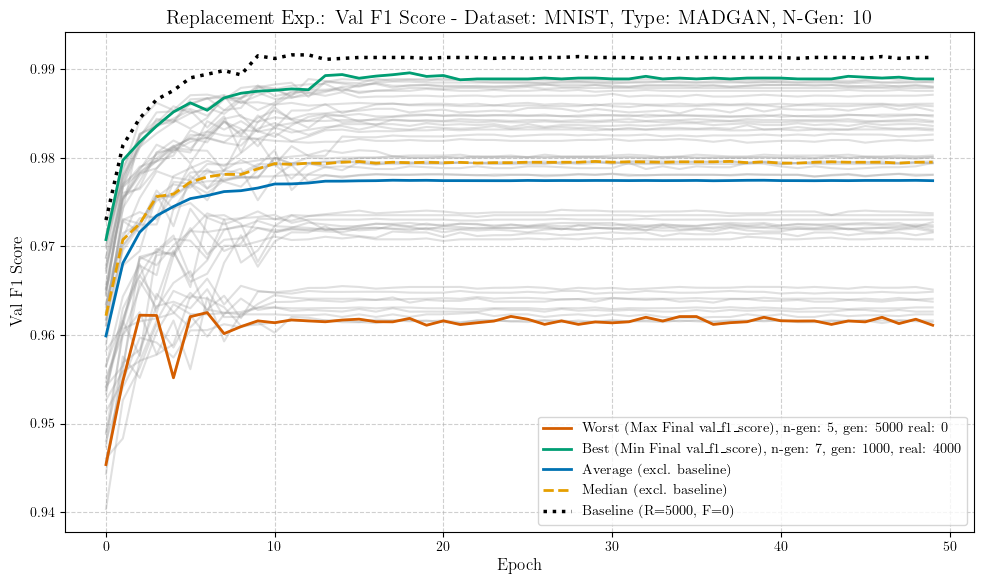
\includegraphics[width=\textwidth]{abb/strat_classifier_performance/MNIST_STRATIFIED_CLASSIFIERS_MADGAN_NEW/replacement_experiments/val_f1_score_MADGAN_MNIST_n_gen_10_all.png}
		\caption{F1 Score on MNIST over 50 epochs. Augmentation technique: MADGAN (K=10)} 
        \label{fig:res_replacement_mnist_tda_vs_madgan__madgan}
	\end{subfigure}
	\begin{subfigure}{.85\textwidth}
		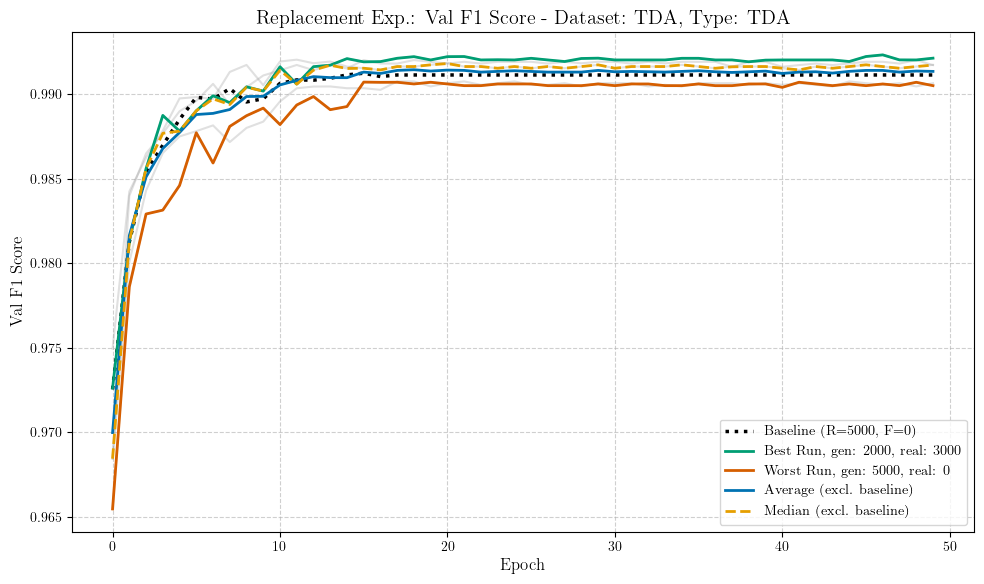
\includegraphics[width=\textwidth]{abb/strat_classifier_performance/tda_mnist/replacement_experiments/val_f1_score_tda_mnist_mnist_all.png}
		\caption{F1 Score on MNIST over 50 epochs. Augmentation Technique: TDA} 
        \label{fig:res_replacement_mnist_tda_vs_madgan__tda}
	\end{subfigure}
%%%%%%%%%%%%%%
\end{figure}

\begin{table}[H]
	\vspace{-1.5em}
	\centering
	\begin{tabular}{|c|c|c|c|}
		\hline
		Run Type & Experiment & Val F1 \\ \hline
		best & \(G_{10, 7}\), R:4000, F:1000 & $0.9889$\\ \hline
		worst & \(G_{10, 5}\), R:0, F:5000 & $0.9611$\\ \hline
		median & - & $0.9795$\\ \hline
		average & - & $0.9774$
		\\ \hline
	\end{tabular}
    \caption{Final F1 Scores after 50 epochs. Augmentation technique: MADGAN}
        \label{tab:res_replacement_mnist_tda_vs_madgan__madgan}
\end{table}
\begin{table}[H]
	\centering
	\vspace{-1.5em}
	\begin{tabular}{|c|c|c|c|c|}
		\hline
		Run Type & Metric & Performance \\ \hline
		best & TDA (R:3000, F:2000) & $0.9922$\\ \hline
		worst & TDA (R:0, F:5000) & $0.9905$\\ \hline
		median & TDA & $0.9917$\\ \hline
		average & TDA & $0.9914$
		\\ \hline
	\end{tabular}
    \caption{Final F1 Scores after 50 epochs. Augmentation technique: TDA}
        \label{tab:res_replacement_mnist_tda_vs_madgan__tda}
\end{table}

The results for TDA, shown in figure \ref{fig:res_replacement_mnist_tda_vs_madgan__tda} and summarized in table \ref{tab:res_replacement_mnist_tda_vs_madgan__tda}. The graphs in the corresponding figure show all out rapid convergence and a stable training over the $50$ epochs. With a small spread of the results, all replacement ratios \\\(\left[ (R:5000, F:0), ..., (R:0, F:5000) \right]\) consistently result in excellent performance with an average F1 score of $0.9914$. The best and worst results are close to the average and both are over $0.99$, only differing in the third decimals. This leads to the conclusion that replacing training images for a classifier with modified images via traditional methods had minimal negative impact on the classifiers' performance, measured on the validation set via the F1 score. It is to point out, that the best, average and median performance surpassed the baseline allowing the conclusion that the replacement of real images with their augmented counterpart had a positive impact on average.

The performance using GDA with samples form MADGAN (K=10) model is presented in Figure \ref{fig:res_replacement_mnist_tda_vs_madgan__madgan} and Table \ref{tab:res_replacement_mnist_tda_vs_madgan__madgan}. It is important to note again, that the figure and the summary statistics encompass results across the 10 individual generators and across all replacement ratios resulting in a total of $60$ total classifiers. The graph shows convergence to a slightly lower F1 scores, compared to those from TDA. Here, the conclusion can be drawn that the replacement of real with augmented images resulted in an overall negative impact. The summary table quantifies this fact: the average final F1 score across ratios and generators is $0.9775$, which is significantly lower than the average of the traditional augmentation. While the best setup (\(G_{10,7}, R:4000, F:1000\)) reached a good score: $0.9889$; it is lower than the average performance across the different ratios in the TDA experiment. Even the worst performing classifier in the TDA experiment is better than the best score for GDA in this case. 

In direct comparison, the TDA consistently outperforms GDA (with its best resulting setting, MADGAN (K=10)) in this replacement scenario. Replacing the real data with synthetic lead to a noticeable degradation of the classifiers' performance on the validation set. Taking the results from question 1 into account (\ref{exp_results_ans_q1}), even the MADGAN setup resulting in the best FID score are not as effective as traditional augmented real data, when substituting the real samples in the training set. 

\newpage
\noindent\textbf{Expansion Experiment, Dataset: MNIST}
\begin{figure}[H]
	\centering
	\begin{subfigure}{.85\textwidth}
		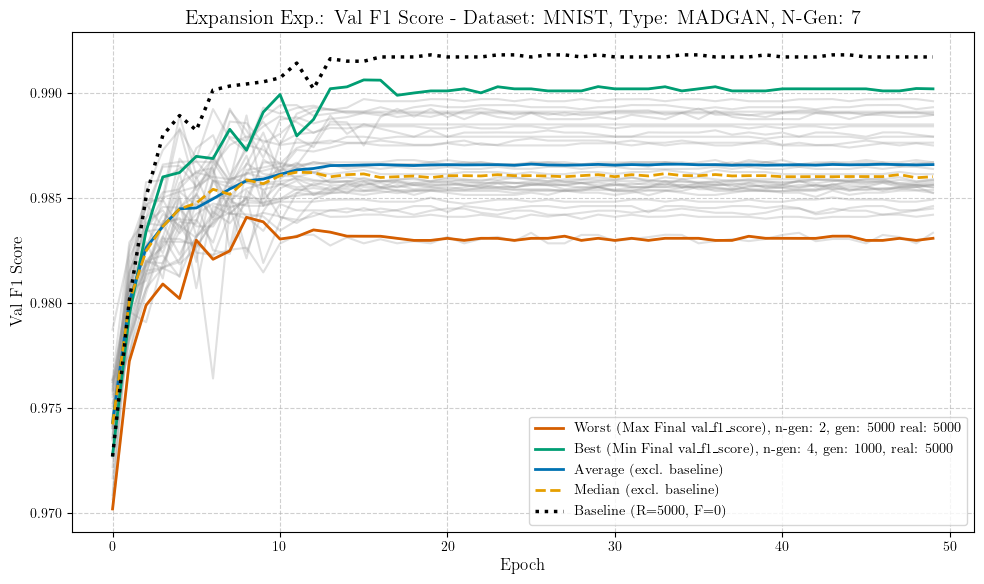
\includegraphics[width=\textwidth]{abb/strat_classifier_performance/MNIST_STRATIFIED_CLASSIFIERS_MADGAN_NEW/expansion_experiments/val_f1_score_MADGAN_MNIST_n_gen_7_all.png}
		\caption{F1 Score on MNIST over 50 epochs. Augmentation technique: MADGAN (K=7)} 
        \label{fig:res_expansion_mnist_tda_vs_madgan__madgan}
	\end{subfigure}
	\begin{subfigure}{.85\textwidth}
		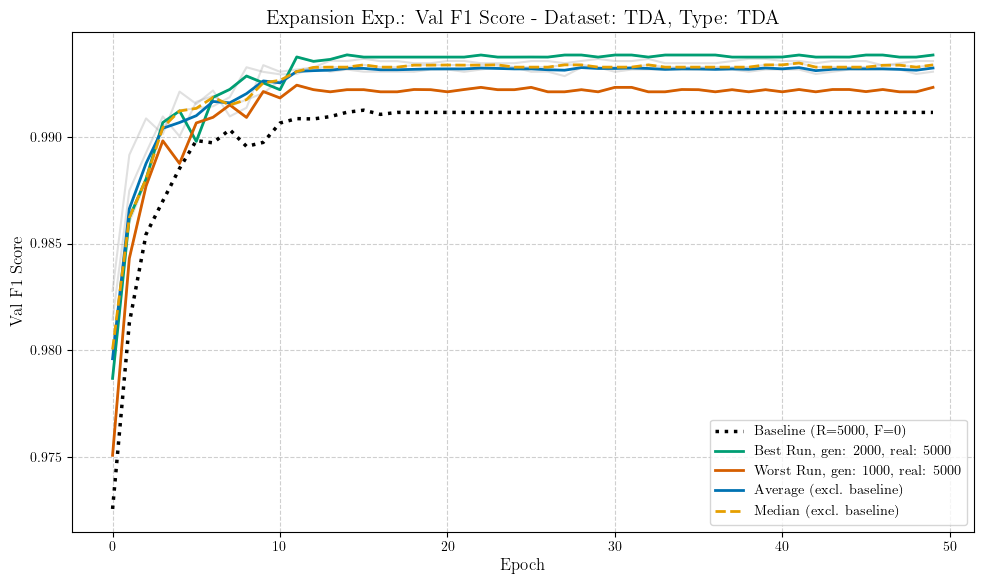
\includegraphics[width=\textwidth]{abb/strat_classifier_performance/tda_mnist/expansion_experiments/val_f1_score_tda_mnist_mnist_all.png}
		\caption{F1 Score on MNIST over 50 epochs. Augmentation Technique: TDA} 
        \label{fig:res_expansion_mnist_tda_vs_madgan__tda}
	\end{subfigure}
%%%%%%%%%%%%%%
\end{figure}

\begin{table}[H]
	\vspace{-1.5em}
	\centering
	\begin{tabular}{|c|c|c|c|}
		\hline
		Run Type & Experiment & Val F1 \\ \hline
		best & \(G_{7, 4}\), R:5000, F:1000 & $0.9902$\\ \hline
		worst & \(G_{7, 2}\), R:5000, F:5000 & $0.9831$\\ \hline
		median & - & $0.9860$\\ \hline
		average & - & $0.9866$
		\\ \hline
	\end{tabular}
    \caption{Final F1 Scores after 50 epochs. Augmentation technique: MADGAN}
        \label{tab:res_expansion_mnist_tda_vs_madgan__madgan}
\end{table}
\begin{table}[H]
	\centering
	\vspace{-1.5em}
	\begin{tabular}{|c|c|c|c|c|}
		\hline
		Run Type & Experiment & Performance \\ \hline
		best & TDA (R:5000, F:2000) & $0.9938$\\ \hline
		worst & TDA (R:5000, F: 1000) & $0.9923$\\ \hline
		median & TDA & $0.9934$\\ \hline
		average & TDA & $0.9932$
		\\ \hline
	\end{tabular}
    \caption{Final F1 Scores after 50 epochs. Augmentation technique: TDA}
        \label{tab:res_expansion_mnist_tda_vs_madgan__tda}
\end{table}

The results using TDA (Table \ref{tab:res_expansion_mnist_tda_vs_madgan__tda}) show consistently high performance. The average final F1 score across all expansion levels (adding 0 to 5,000 augmented samples per class) is 0.9932, with minimal variation between the best (0.9938, achieved when adding 2,000 augmented samples) and worst (0.9923) cases. This indicates that expanding the dataset with traditionally augmented samples maintains, and perhaps very slightly improves, the already high baseline performance on MNIST.

In contrast, using GDA with samples generated by the MADGAN (K=7) model did not yield performance improvements over the baseline trained only on real data. To be noted explicitly, none of the expansion experiments using MADGAN GDA surpassed the baseline performance level (see: \ref{app_strat_class_performance_madgan_mnist}). The summary statistics in Table \ref{tab:res_expansion_mnist_tda_vs_madgan__madgan}, which cover results across all 7 generators and all expansion ratios, confirm this. The average final F1 score is 0.9866, noticeably lower than the TDA results. The best-performing run across all generators and expansion levels only reached 0.9902 (using generator \(G_{7,4}\) when adding 1,000 synthetic samples), which is below even the worst TDA result. Performance tended to decrease as more synthetic data was added, with the lowest score (0.9831) occurring when the maximum of 5,000 synthetic samples per class were added (using generator \(G_{7,2}\)).

Comparing the two augmentation strategies in the expansion scenario, TDA is clearly superior on MNIST in this setup. Expanding the dataset with traditionally augmented data maintains excellent performance, whereas expanding with MADGAN-generated synthetic data fails to improve over the real-data baseline and leads to lower overall performance. This suggests that the synthetic samples from MADGAN (K=7), despite the model potentially having good generative scores, dilute rather than enhance the training data quality when added to the real MNIST dataset for this downstream classification task.


\newpage
\noindent\textbf{Replacement Experiment, Dataset: Fashion-MNIST}
\begin{figure}[H]
	\centering
	\begin{subfigure}{.85\textwidth}
		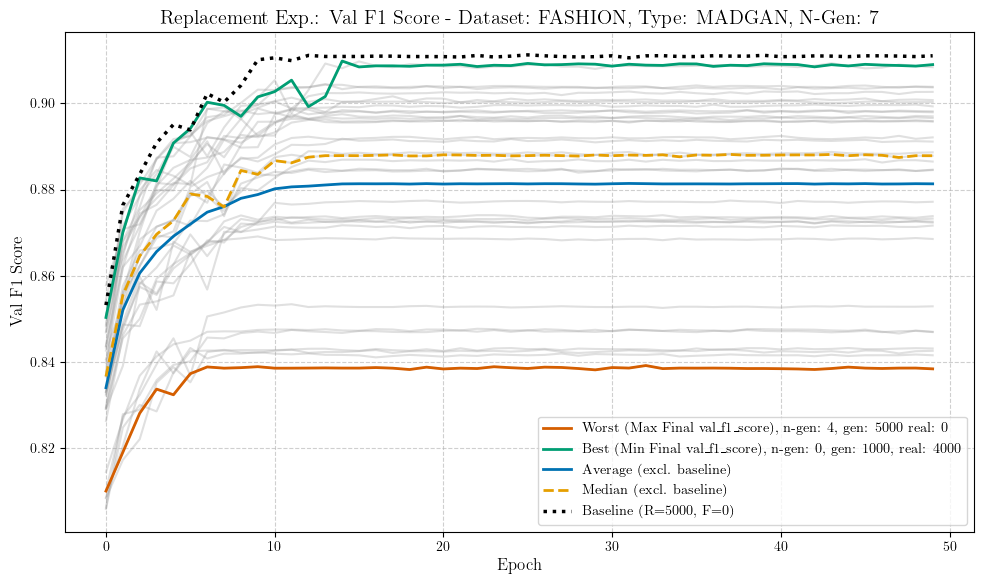
\includegraphics[width=\textwidth]{abb/strat_classifier_performance/FASHION_STRATIFIED_CLASSIFIERS_MADGAN_NEW/replacement_experiments/val_f1_score_MADGAN_FASHION_n_gen_7_all.png}
		\caption{F1 Score on FASHION over 50 epochs. Augmentation tech.: MADGAN (K=7)} 
        \label{fig:res_replacement_fashion_tda_vs_madgan__madgan}
	\end{subfigure}
	\begin{subfigure}{.85\textwidth}
		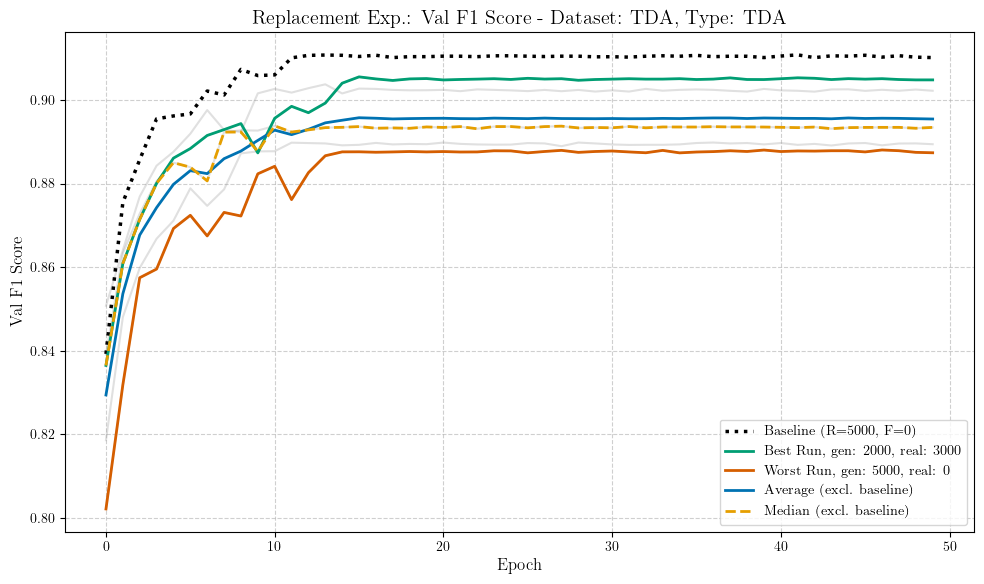
\includegraphics[width=\textwidth]{abb/strat_classifier_performance/tda_fashion_mnist/replacement_experiments/val_f1_score_tda_fashion_mnist_fashion_all.png}
		\caption{F1 Score on FASHION over 50 epochs. Augmentation Technique: TDA} 
        \label{fig:res_replacement_fashion_tda_vs_madgan__tda}
	\end{subfigure}
%%%%%%%%%%%%%%
\end{figure}

\begin{table}[H]
	\vspace{-1.5em}
	\centering
	\begin{tabular}{|c|c|c|c|}
		\hline
		Run Type & Experiment & Val F1 \\ \hline
		best & \(G_{7, 2}\), R:4000, F:1000 & $0.9079$\\ \hline
		worst & \(G_{7, 0}\), R:0, F:5000 & $0.3419$\\ \hline
		median & - & $0.8927$\\ \hline
		average & - & $0.7993$
		\\ \hline
	\end{tabular}
    \caption{Final F1 Scores after 50 epochs. Augmentation tech.: MADGAN (K=7)}
        \label{tab:res_replacement_fashion_tda_vs_madgan__madgan}
\end{table}
\begin{table}[H]
	\centering
	\vspace{-1.5em}
	\begin{tabular}{|c|c|c|c|c|}
		\hline
		Run Type & Experiment & Val F1 \\ \hline
		best & TDA (R:3000, F:2000) & $0.9048$\\ \hline
		worst & TDA (R:0, F:5000) & $0.8874$\\ \hline
		median & TDA & $0.8934$\\ \hline
		average & TDA & $0.8955$
		\\ \hline
	\end{tabular}
    \caption{Final F1 Scores after 50 epochs. Augmentation technique: TDA}
        \label{tab:res_replacement_fashion_tda_vs_madgan__tda}
\end{table}
For TDA (Table \ref{tab:res_replacement_fashion_tda_vs_madgan__tda}), the results indicate reasonably strong and relatively stable classifier performance as real data is replaced by traditionally augmented samples. The average final F1 score across all replacement ratios is 0.8955. Performance degrades moderately as more real data is substituted, with the best score (0.9048) observed at a mix of 3000 real and 2000 augmented samples per class, and the worst score (0.8874) occurring when using only augmented data (0 real, 5000 augmented). The overall range is narrow, suggesting TDA provides consistent results.

The MADGAN (K=7) GDA results (Table \ref{tab:res_replacement_fashion_tda_vs_madgan__madgan}) reveal a much higher degree of variability. These summary statistics encompass results across all 7 individual generators and all replacement ratios. Notably, the best-performing run (generator \(G_{7,2}\) with 4000 real / 1000 fake samples) achieved an F1 score of 0.9079, slightly surpassing the best TDA result. However, extreme inconsistency offsets this potential advantage. The worst-performing run (generator \(G_{7,0}\) using only synthetic data) yielded a drastically low F1 score of 0.3419, far below the worst TDA score. This disparity heavily impacts the average F1 score for MADGAN GDA, bringing it down to 0.7993, significantly lower than the TDA average. Interestingly, the median F1 score for MADGAN GDA (0.8927) is quite close to the TDA median (0.8934), suggesting that while the average is poor due to outliers, typical performance might be closer to TDA.

In direct comparison for the replacement scenario on Fashion-MNIST, TDA offers more reliable and consistent performance. While MADGAN GDA demonstrates the potential to slightly exceed TDA's peak performance under specific optimal conditions (best generator, limited replacement), it suffers from extreme variability. Relying solely on synthetic data from weaker generators leads to a catastrophic performance drop, making MADGAN GDA a much less robust strategy on average compared to TDA when replacing real data in this setup.


\newpage
\noindent\textbf{Expansion Experiment, Dataset: Fashion-MNIST}
\begin{figure}[H]
	\centering
	\begin{subfigure}{.85\textwidth}
		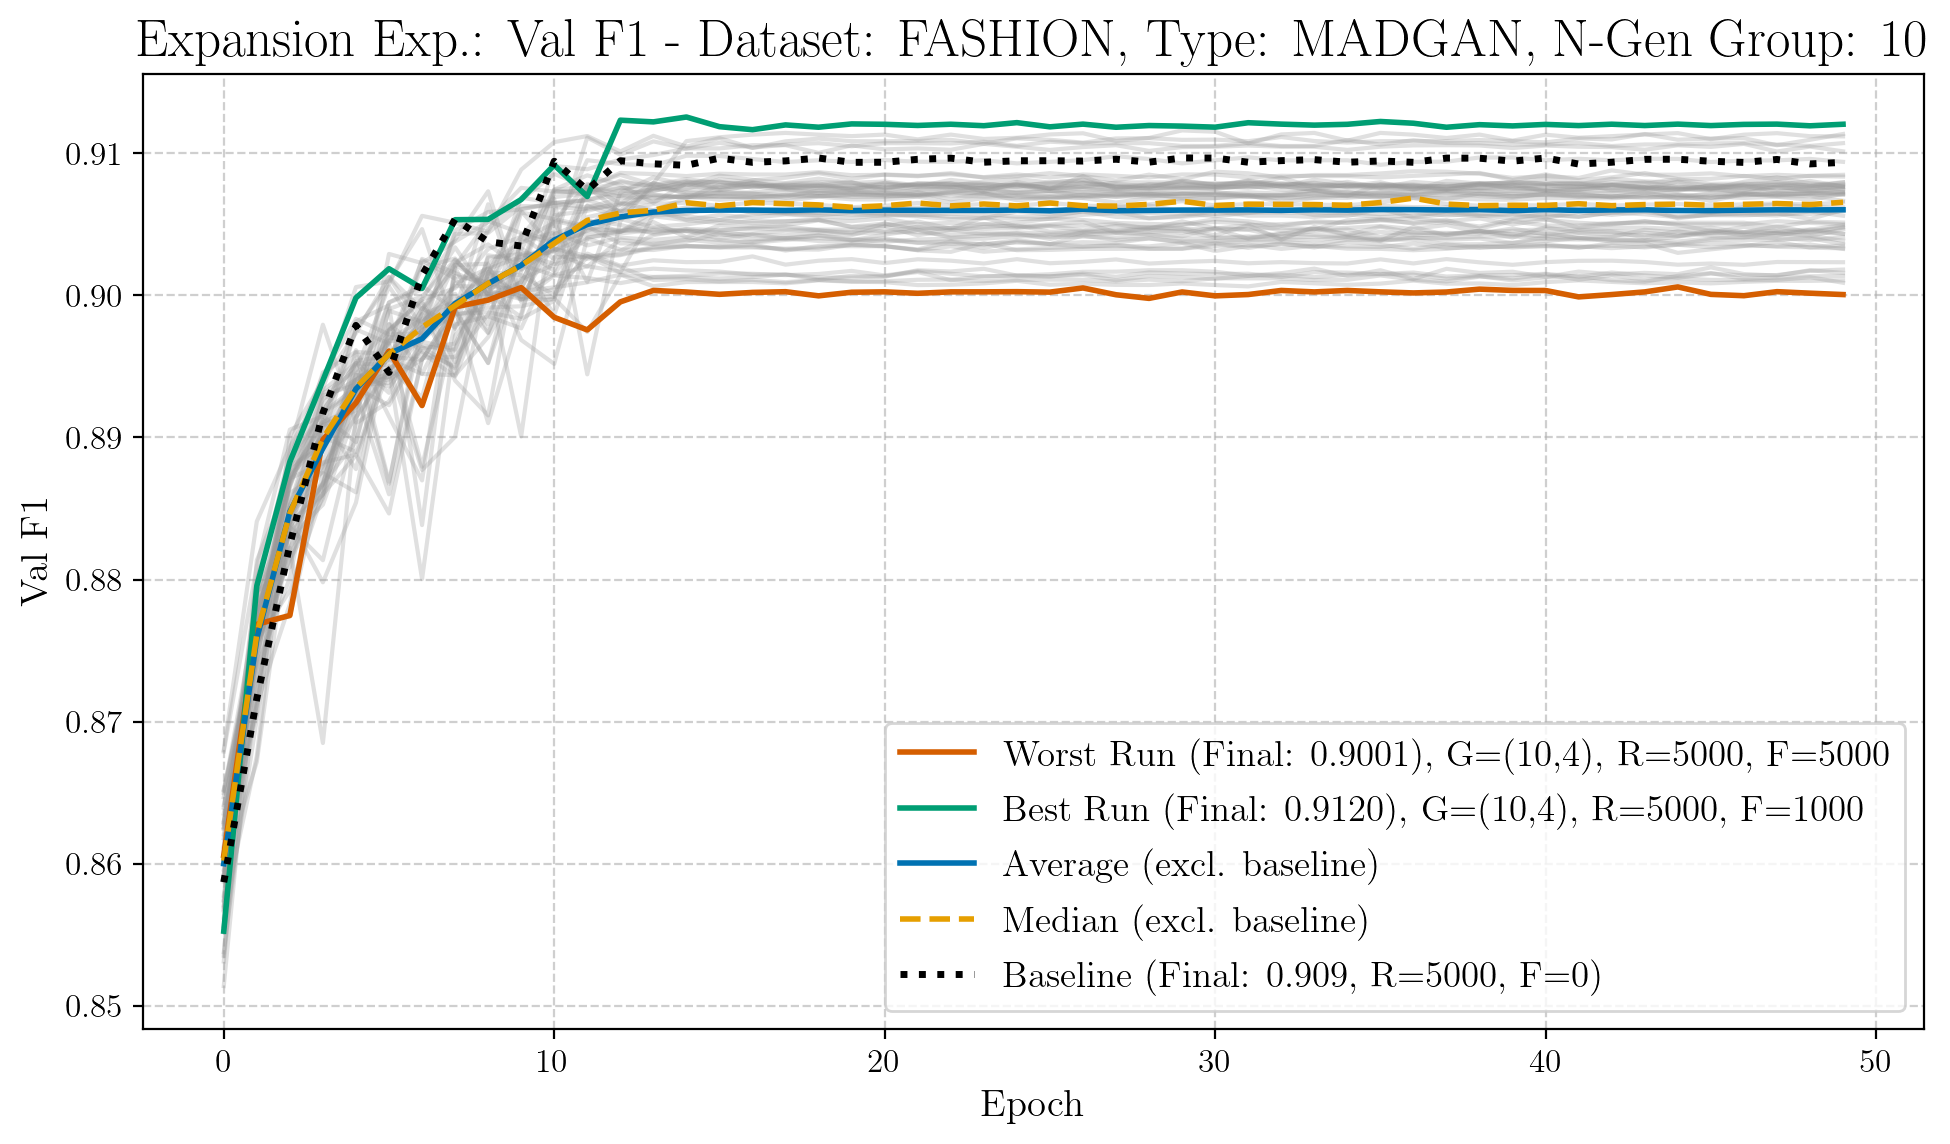
\includegraphics[width=\textwidth]{abb/strat_classifier_performance/FASHION_STRATIFIED_CLASSIFIERS_MADGAN_NEW/expansion_experiments/val_f1_score_MADGAN_FASHION_n_gen_10_all.png}
		\caption{F1 Score on FASHION over 50 epochs. Augmentation tech.: MADGAN (K=10)} 
        \label{fig:res_expansion_fashion_tda_vs_madgan__madgan}
	\end{subfigure}
	\begin{subfigure}{.85\textwidth}
		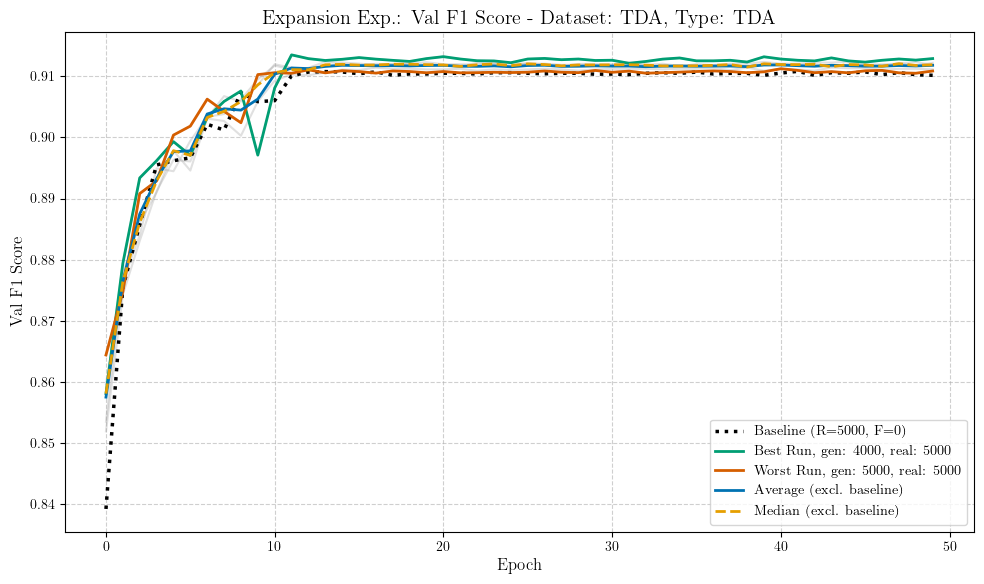
\includegraphics[width=\textwidth]{abb/strat_classifier_performance/tda_fashion_mnist/expansion_experiments/val_f1_score_tda_fashion_mnist_fashion_all.png}
		\caption{F1 Score on FASHION over 50 epochs. Augmentation Technique: TDA} 
        \label{fig:res_expansion_fashion_tda_vs_madgan__tda}
	\end{subfigure}
%%%%%%%%%%%%%%
\end{figure}

\begin{table}[H]
	\vspace{-1.5em}
	\centering
	\begin{tabular}{|c|c|c|c|}
		\hline
		Run Type & Experiment & Val F1 \\ \hline
		best & \(G_{10, 4}\), R:5000, F:1000 & $0.9120$\\ \hline
		worst & \(G_{10, 4}\), R:5000, F:5000 & $0.9001$\\ \hline
		median & - & $0.9066$\\ \hline
		average & - & $0.9060$
		\\ \hline
	\end{tabular}
    \caption{Final F1 Scores after 50 epochs. Augmentation tech.: MADGAN (K=X)}
        \label{tab:res_expansion_fashion_tda_vs_madgan__madgan}
\end{table}
\begin{table}[H]
	\centering
	\vspace{-1.5em}
	\begin{tabular}{|c|c|c|c|c|}
		\hline
		Run Type & Experiment & Val F1 \\ \hline
		best & TDA (R:5000, F:4000) & $0.9129$\\ \hline
		worst & TDA (R:5000, F:5000) & $0.9108$\\ \hline
		median & TDA & $0.9119$\\ \hline
		average & TDA & $0.9118$
		\\ \hline
	\end{tabular}
    \caption{Final F1 Scores after 50 epochs. Augmentation technique: TDA}
        \label{tab:res_expansion_fashion_tda_vs_madgan__tda}
\end{table}

The results indicate that data expansion is beneficial on Fashion-MNIST for both augmentation techniques, unlike the observations on MNIST where MADGAN GDA did not surpass the baseline. Using TDA (Table \ref{tab:res_expansion_fashion_tda_vs_madgan__tda}), adding augmented samples improves performance over baseline (R:5000/F:0), achieving a peak F1 score of $0.9129$ when adding $4.000$ augmented samples per class. Performance remains very high and stable across different expansion levels, with an average F1 of $0.9118$ and even the worst case (adding $5.000$ samples) scoring $0.9108$.

Similarly, expansion using MADGAN (K=10) GDA also demonstrates the potential to improve performance over the baseline. The summary statistics in Table \ref{tab:res_expansion_fashion_tda_vs_madgan__madgan}, covering results across all 10 generators and expansion ratios, show a best-case F1 score of $0.9120$ (achieved by generator \(G_{10,4}\) when adding $1.000$ synthetic samples). This peak performance is very close to the TDA peak and suggests GDA can be effective in this scenario. However, MADGAN GDA performance is slightly less consistent than TDA. The average F1 score ($0.9060$) and median ($0.9066$) are marginally lower than TDA's averages. Furthermore, performance degrades more noticeably when adding the maximum number of synthetic samples, with the worst run dropping to $0.9001$, below TDA's worst case. The variability across generators and ratios, while present, is considerably less extreme than observed in the Fashion-MNIST replacement experiment.

In direct comparison for the expansion scenario on Fashion-MNIST, both TDA and MADGAN GDA (K=10) show benefits over using only the original real data. TDA maintains a slight edge, providing marginally higher peak performance and greater stability, especially when large amounts of augmented data are added. MADGAN GDA is highly competitive, achieving a peak performance nearly identical to TDA's, but exhibiting slightly lower average scores and greater performance degradation when maximally expanded. This suggests MADGAN GDA is a viable expansion technique on Fashion-MNIST, though TDA remains slightly more robust.

\newpage
\subsubsection[Question 3]{MADGAN GDA vs. Deep Convolutional/Conditional GAN GDA} \label{exp_results_ans_q3} 
In the foregoing chapter (\ref{exp_results_ans_q2}), the most successful setting for the MADGAN architecture has been set. Following, the same settings for the respective dataset and the corresponding experimental setup (replacement, expansion) will be used to compare against deep convolutional and conditional GANs
\newpage

\noindent\textbf{Replacement Experiment, Dataset: MNIST}
\begin{figure}[H] 
	\centering
	\begin{subfigure}{.85\textwidth}
		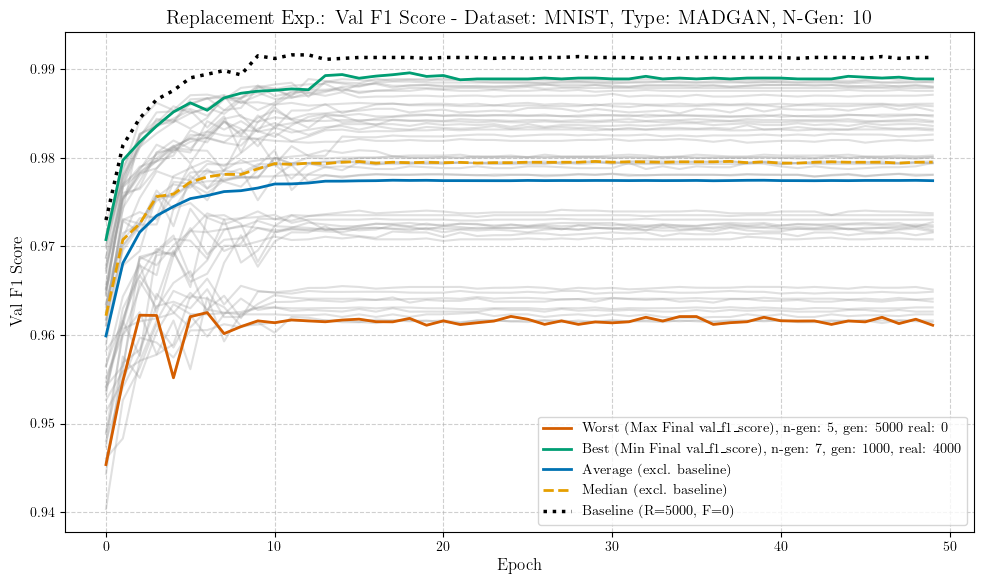
\includegraphics[width=\textwidth]{abb/strat_classifier_performance/MNIST_STRATIFIED_CLASSIFIERS_MADGAN_NEW/replacement_experiments/val_f1_score_MADGAN_MNIST_n_gen_10_all.png}
		\caption{F1 Score on MNIST over 50 epochs. Augmentation technique: MADGAN (K=10)} 
        \label{fig:res_replacement_mnist_tda_vs_madgan__madgan}
	\end{subfigure}
	\begin{subfigure}{.85\textwidth}
		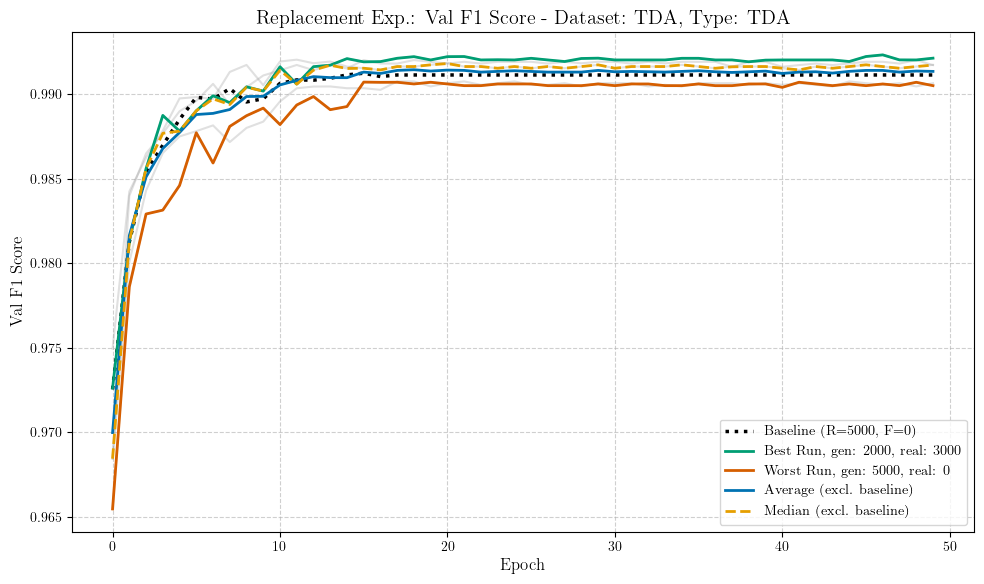
\includegraphics[width=\textwidth]{abb/strat_classifier_performance/tda_mnist/replacement_experiments/val_f1_score_tda_mnist_mnist_all.png}
		\caption{F1 Score on MNIST over 50 epochs. Augmentation Technique: TDA} 
        \label{fig:res_replacement_mnist_tda_vs_madgan__tda}
	\end{subfigure}
%%%%%%%%%%%%%%
\end{figure}

\begin{table}[H]
	\vspace{-1.5em}
	\centering
	\begin{tabular}{|c|c|c|c|}
		\hline
		Run Type & Experiment & Val F1 \\ \hline
		best & \(G_{10, 7}\), R:4000, F:1000 & $0.9889$\\ \hline
		worst & \(G_{10, 5}\), R:0, F:5000 & $0.9611$\\ \hline
		median & - & $0.9795$\\ \hline
		average & - & $0.9774$
		\\ \hline
	\end{tabular}
    \caption{Final F1 Scores after 50 epochs. Augmentation technique: MADGAN}
        \label{tab:res_replacement_mnist_tda_vs_madgan__madgan}
\end{table}
\begin{table}[H]
	\centering
	\vspace{-1.5em}
	\begin{tabular}{|c|c|c|c|c|}
		\hline
		Run Type & Metric & Performance \\ \hline
		best & TDA (R:3000, F:2000) & $0.9922$\\ \hline
		worst & TDA (R:0, F:5000) & $0.9905$\\ \hline
		median & TDA & $0.9917$\\ \hline
		average & TDA & $0.9914$
		\\ \hline
	\end{tabular}
    \caption{Final F1 Scores after 50 epochs. Augmentation technique: TDA}
        \label{tab:res_replacement_mnist_tda_vs_madgan__tda}
\end{table}


\subsubsection[Question 4]{MADGAN GDA vs. cMADGAN GDA Performance}      \label{exp_results_ans_q4} 
 

\subsubsection[Question 5]{Impact of MADGAN Generator Count}            \label{exp_results_ans_q5} 
 


\newpage
